\documentclass[12pt,a4paper]{article}
\usepackage[utf8]{inputenc}
\usepackage{times}
\usepackage{amsmath}
\usepackage{amssymb}
\usepackage{graphicx}
\usepackage{cite}
\usepackage{url}
\usepackage{hyperref}
\usepackage{geometry}
\usepackage{setspace}
\usepackage{indentfirst}
\usepackage{fancyhdr} % For page numbers
\usepackage[font={it,footnotesize}]{caption} % For caption formatting (10pt)
\usepackage{sectsty} % For section title formatting
\usepackage{booktabs} % For professional quality tables
\usepackage{tikz}
\usetikzlibrary{shapes.geometric, arrows, positioning, fit, calc}

% Set section/subsection title format (12pt, bold)
\sectionfont{\fontsize{12}{15}\selectfont\bfseries}
\subsectionfont{\fontsize{12}{15}\selectfont\bfseries}

% Set page number to bottom center
\pagestyle{fancy}
\fancyhf{}
\fancyfoot[C]{\thepage}
\renewcommand{\headrulewidth}{0pt}

% Set page margins
\geometry{left=2.54cm,right=2.54cm,top=2.54cm,bottom=2.54cm}

% Set line spacing to 1.5
\renewcommand{\baselinestretch}{1.5}

% Set paragraph indentation
\setlength{\parindent}{0.5cm}

% Title formatting
\title{\fontsize{14}{17}\selectfont\textbf{Advances in Deep Learning for Remote Sensing Image Classification: A Comprehensive Review}}
\author{[Your Full Name]\\
[Your School/College]\\
Northwestern Polytechnical University\\
Xi'an, Shaanxi, China\\
\texttt{[your.email@mail.nwpu.edu.cn]}}
\date{}

\begin{document}

\maketitle

\begin{abstract}
Deep learning has revolutionized remote sensing image classification, with convolutional neural networks (CNNs) demonstrating remarkable performance across diverse applications. This review examines recent advances in deep learning architectures for remote sensing, focusing on multi-scale feature extraction, attention mechanisms, and transfer learning. We analyze developments in three key areas: scene classification, object detection, and semantic segmentation. Critical challenges including limited training data, computational efficiency, and domain-specific adaptations are discussed. Based on analysis of recent research, we identify promising directions including self-supervised learning, multi-modal fusion, and lightweight architectures. This review provides insights into current state-of-the-art methods and future research opportunities in this rapidly evolving field.
\end{abstract}

\textbf{Keywords:} Deep learning, Remote sensing, Image classification, Convolutional neural networks, Scene classification, Object detection

\section{Introduction}
\label{sec:introduction}

Remote sensing technology has undergone remarkable advancement in recent years, with integrated space-air-ground observation platforms generating unprecedented volumes of imagery data. These high-resolution remote sensing images contain rich spectral, spatial, and temporal information that is crucial for various applications, including land cover mapping, urban planning, disaster monitoring, and environmental management. However, the increasing complexity and scale of remote sensing data present significant challenges for traditional image classification methods.

Conventional remote sensing image classification approaches typically rely on manually designed features such as spectral indices, texture descriptors, and shape characteristics. While these methods have proven effective for certain applications, they often fail to capture the complex nonlinear relationships in high-dimensional remote sensing data, particularly when dealing with diverse land cover types and varying acquisition conditions \cite{cheng2016survey}. Moreover, the feature engineering process is time-consuming and requires substantial domain expertise, making it difficult to adapt to new sensors or application domains.

The emergence of deep learning has revolutionized the field of computer vision and offers new opportunities for remote sensing image analysis \cite{zhu2017deep}. Unlike traditional machine learning methods, deep learning models can automatically learn hierarchical feature representations directly from raw data, eliminating the need for manual feature engineering. Among various deep learning architectures, convolutional neural networks (CNNs) have demonstrated exceptional performance in image classification tasks by effectively capturing spatial patterns and contextual information.

In recent years, researchers have increasingly applied CNNs to remote sensing image classification, achieving remarkable improvements in accuracy and robustness \cite{liu2019learning}. However, remote sensing images present unique challenges compared with natural images, including multi-spectral bands, varying spatial resolutions, complex scene compositions, and limited labeled training data \cite{cheng2016survey}. These challenges have motivated the development of specialized CNN architectures and training strategies specifically designed for remote sensing applications.

This paper provides a comprehensive review of recent advances in deep learning for remote sensing image classification, focusing on developments from 2020 to 2023. We examine key improvements in CNN architectures, training methodologies, and application-specific adaptations. The review is organized as follows: Section 2 discusses the background and fundamental concepts of CNNs for remote sensing. Section 3 reviews recent developments in CNN architectures for remote sensing applications. Section 4 presents three major application areas: scene classification, object detection, and semantic segmentation. Section 5 discusses current challenges and future research directions. Finally, Section 6 concludes the paper with a summary of key findings.

\section{Background}
\label{sec:background}

\subsection{Convolutional Neural Networks Fundamentals}
Convolutional neural networks are deep learning architectures specifically designed for processing grid-like data, such as images. The core components of a CNN include convolutional layers, pooling layers, fully connected layers, and activation functions. 

Convolutional layers apply learnable filters to input images to extract local features, with each filter detecting specific patterns such as edges, textures, or shapes. The key advantages of convolutional operations include parameter sharing (reducing the number of trainable parameters) and local connectivity (capturing spatial relationships). Pooling layers reduce the spatial dimensions of feature maps while preserving important information, making the network more robust to small translations and reducing computational requirements.

Fully connected layers integrate high-level features extracted by convolutional and pooling layers to perform final classification or regression tasks. Activation functions introduce non-linearity into the network, enabling it to learn complex relationships between inputs and outputs. Common activation functions include Rectified Linear Units (ReLU), sigmoid, and tanh.

\subsection{CNN Training and Optimization}
CNN training involves minimizing a loss function that measures the discrepancy between predicted outputs and ground truth labels. The training process typically uses backpropagation and gradient-based optimization algorithms such as stochastic gradient descent (SGD) or Adam. 

Several techniques are commonly employed to improve CNN training performance and prevent overfitting, including:
\begin{itemize}
\item \textbf{Data augmentation}: Artificially expanding the training dataset through transformations such as rotation, scaling, and flipping
\item \textbf{Regularization}: Adding constraints to the loss function, such as L1/L2 regularization or dropout, to prevent overfitting
\item \textbf{Batch normalization}: Normalizing layer inputs to reduce internal covariate shift and accelerate training
\item \textbf{Transfer learning}: Utilizing pre-trained models from large-scale datasets and fine-tuning them for specific tasks
\end{itemize}

\subsection{Challenges in Remote Sensing Image Classification}
Remote sensing images present several unique challenges that distinguish them from natural images \cite{zhu2017deep}:

\begin{itemize}
\item \textbf{Multi-spectral information}: Remote sensing images often contain multiple spectral bands beyond RGB, requiring adaptation of CNN architectures to handle additional channels
\item \textbf{Varying spatial resolutions}: Different sensors capture images at different spatial resolutions, affecting the scale of objects and features \cite{cheng2016survey}
\item \textbf{Complex scene compositions}: Remote sensing scenes typically contain multiple objects with complex spatial relationships and varying scales \cite{xia2017aid}
\item \textbf{Limited labeled data}: Acquiring accurately labeled remote sensing data is expensive and time-consuming, leading to small training datasets \cite{zhu2017deep}
\item \textbf{Class imbalance}: Certain land cover classes may be significantly underrepresented in the training data
\end{itemize}

These challenges have motivated the development of specialized CNN architectures and training strategies specifically designed for remote sensing applications, as discussed in the following sections.

\section{Developments in CNN Architectures for Remote Sensing}
\label{sec:developments}

\subsection{Multi-scale Feature Extraction}
Remote sensing images contain objects at multiple scales, from small buildings to large landscape features. Traditional CNN architectures with fixed receptive fields may struggle to capture features across this wide range of scales. Recent developments have focused on incorporating multi-scale feature extraction capabilities.

Pyramid pooling modules have been integrated into CNN architectures to capture features at different spatial scales. These modules apply parallel pooling operations at different scales and concatenate the results, enabling the network to capture both local details and global context. Similarly, atrous spatial pyramid pooling uses dilated convolutions with different dilation rates to expand the receptive field without increasing computational requirements.

Feature pyramid networks introduce top-down pathways and lateral connections to combine high-level semantic features with low-level detailed features. This architecture enables effective detection of objects at different scales by generating feature pyramids with rich semantic information at all levels.

\subsection{Attention Mechanisms}
Attention mechanisms have become increasingly popular in remote sensing image classification, enabling networks to focus on the most relevant regions and features. These mechanisms can be broadly categorized into spatial attention and channel attention.

Spatial attention modules generate attention maps that highlight important spatial regions in the feature maps. These modules help the network focus on discriminative regions while ignoring irrelevant background areas. Channel attention modules model the interdependencies between different feature channels, emphasizing informative channels and suppressing less useful ones.

Convolutional block attention modules combine both spatial and channel attention in a sequential manner, providing comprehensive attention capabilities. These modules have been shown to improve classification accuracy, particularly for complex remote sensing scenes with multiple object categories.

\subsection{Transfer Learning and Domain Adaptation}
Limited labeled training data in remote sensing has motivated extensive research on transfer learning and domain adaptation techniques \cite{zhu2017deep}. Transfer learning leverages knowledge from large-scale natural image datasets (such as ImageNet) and adapts it to remote sensing tasks.

Fine-tuning pre-trained CNN models has become a standard approach in remote sensing image classification. This involves initializing network weights with parameters learned from large datasets and then updating them on the target remote sensing dataset. Fine-tuning typically achieves better performance than training from scratch, particularly with limited training data.

Domain adaptation techniques address the domain shift between natural images and remote sensing images. These methods align feature distributions between source and target domains through adversarial training or discrepancy minimization, enabling better transfer of knowledge across domains.

\subsection{Lightweight Network Designs}
Computational efficiency has become increasingly important for remote sensing applications, particularly for deployment on resource-constrained platforms such as satellites and unmanned aerial vehicles. Lightweight network designs aim to reduce computational requirements while maintaining classification accuracy.

Depthwise separable convolutions decompose standard convolutions into depthwise and pointwise convolutions, significantly reducing computational complexity. MobileNet and its variants utilize this approach to achieve efficient performance on mobile and embedded devices.

Neural architecture search has been applied to automatically design efficient network architectures specifically for remote sensing tasks. These approaches optimize network architectures for specific hardware constraints and performance requirements, often discovering novel designs that outperform manually crafted architectures.

\section{Application Cases}
\label{sec:applications}

This section reviews three major application areas where deep learning has been successfully applied. A summary of these tasks, their common architectures, and key challenges is provided in Table~\ref{tab:task_comparison}.

\begin{table}[h!]
\centering
\caption{Comparison of Major Deep Learning Tasks in Remote Sensing.}
\label{tab:task_comparison}
\resizebox{\textwidth}{!}{%
\begin{tabular}{@{}llll@{}}
\toprule
\textbf{Task} & \textbf{Description} & \textbf{Common Architectures} & \textbf{Key Challenges} \\ \midrule
Scene Classification & Categorize an image based on its overall content. & CNNs with global average pooling, Multi-scale networks & Intra-class diversity, Inter-class similarity \\
Object Detection & Locate and identify specific objects (e.g., vehicles). & Faster R-CNN, YOLO, SSD, Rotated BBox methods & Small object sizes, Varying orientations, Dense objects \\
Semantic Segmentation & Assign a class label to every pixel in an image. & FCN, U-Net, DeepLab, Encoder-Decoder models & Fine detail preservation, Class imbalance, Edge refinement \\ \bottomrule
\end{tabular}%
}
\end{table}


\subsection{Scene Classification}
Scene classification involves categorizing remote sensing images into predefined land use or land cover categories based on their overall content. This task is challenging due to the complex composition of remote sensing scenes, which typically contain multiple objects with varying spatial arrangements \cite{xia2017aid}.

Recent advances in scene classification have focused on capturing both global context and local object details \cite{zeng2018improving}. Global context features capture the overall scene layout and land cover distribution, while local object features provide detailed information about individual elements within the scene.

Multi-scale feature fusion approaches combine features extracted at different spatial resolutions to improve scene classification accuracy. These approaches typically use feature pyramid structures or parallel convolutional pathways with different receptive field sizes to capture both fine-grained details and coarse-grained context.

Attention mechanisms have been widely applied to scene classification to focus on discriminative regions within complex scenes. These mechanisms help filter out irrelevant background areas and emphasize informative regions that contribute to scene understanding.

\subsection{Object Detection}
Object detection in remote sensing images involves locating and identifying specific objects such as buildings, vehicles, or aircraft \cite{cheng2016survey}. This task is challenging due to the small size of objects, varying orientations, and complex backgrounds in remote sensing images \cite{zhang2016weakly}.

Two-stage object detection methods, such as Faster R-CNN, generate region proposals and then classify each region. These methods typically achieve high accuracy but may be computationally expensive for large remote sensing images \cite{deng2017enhanced}.

Single-stage object detection methods, such as YOLO and SSD, perform detection in a single pass through the network, offering better computational efficiency. These methods have been adapted for remote sensing applications through modifications such as multi-scale feature pyramids and anchor box designs optimized for remote sensing objects.

Orientation-aware object detection methods address the challenge of rotated objects in remote sensing images by incorporating orientation estimation into the detection framework. These methods typically use rotated bounding boxes or angle prediction modules to improve detection accuracy for objects with arbitrary orientations.

\subsection{Semantic Segmentation}
Semantic segmentation assigns class labels to each pixel in remote sensing images, providing detailed land cover maps. This task is essential for applications such as urban planning, agricultural monitoring, and environmental assessment \cite{maggiori2017end}.

Fully convolutional networks (FCN) replace fully connected layers in traditional CNNs with convolutional layers, enabling pixel-level prediction for images of arbitrary size. FCN-based approaches have been widely adapted for remote sensing semantic segmentation through modifications such as multi-scale feature fusion and skip connections.

Encoder-decoder architectures, such as U-Net and DeepLab, capture multi-scale context through symmetric encoder and decoder pathways. The U-Net structure, with its characteristic skip connections, is particularly effective at preserving fine details by merging deep, semantic features with shallow, high-resolution features (see Figure~\ref{fig:unet_architecture}). These architectures have proven effective for remote sensing semantic segmentation by combining high-resolution features with semantic context \cite{liu2019learning}.

\begin{figure}[h!]
\centering
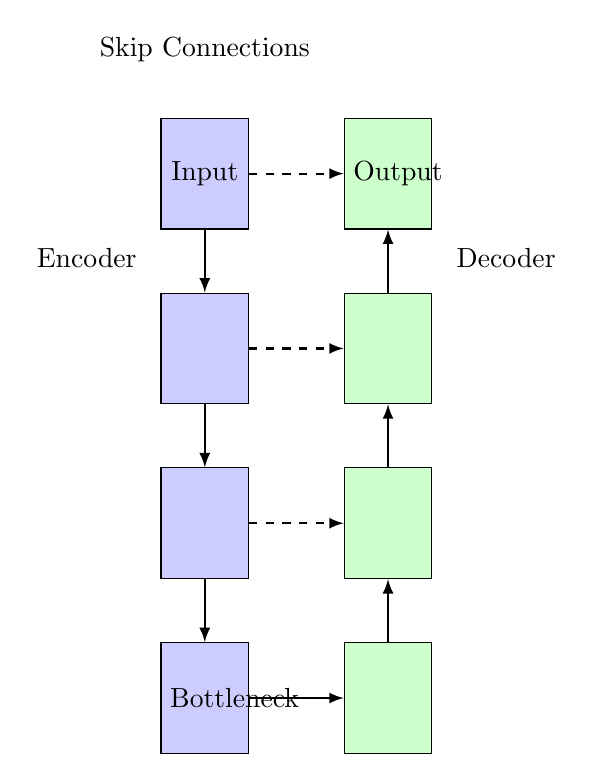
\begin{tikzpicture}[
    node distance=0.8cm and 1.2cm,
    block/.style={rectangle, draw, fill=blue!20, text width=2.5em, text centered, minimum height=4em},
    dblock/.style={rectangle, draw, fill=green!20, text width=2.5em, text centered, minimum height=4em},
    arrow/.style={-latex, thick}
]
    % Encoder Path
    \node[block] (e1) {Input};
    \node[block, below=of e1] (e2) {};
    \node[block, below=of e2] (e3) {};
    \node[block, below=of e3] (e4) {Bottleneck};

    % Decoder Path
    \node[dblock, right=of e4] (d4) {};
    \node[dblock, above=of d4] (d3) {};
    \node[dblock, above=of d3] (d2) {};
    \node[dblock, above=of d2] (d1) {Output};

    % Connections
    \draw[arrow] (e1) -- (e2);
    \draw[arrow] (e2) -- (e3);
    \draw[arrow] (e3) -- (e4);
    \draw[arrow] (e4) -- (d4);
    \draw[arrow] (d4) -- (d3);
    \draw[arrow] (d3) -- (d2);
    \draw[arrow] (d2) -- (d1);

    % Skip Connections
    \draw[arrow, dashed] (e3.east) to [out=0, in=180] (d3.west);
    \draw[arrow, dashed] (e2.east) to [out=0, in=180] (d2.west);
    \draw[arrow, dashed] (e1.east) to [out=0, in=180] (d1.west);
    
    % Labels
    \node[above=0.2cm of e2, xshift=-1.5cm, align=center] {Encoder};
    \node[above=0.2cm of d2, xshift=1.5cm, align=center] {Decoder};
    \node[above=0.1cm of d2, midway, yshift=1.2cm] {Skip Connections};

\end{tikzpicture}
\caption{A simplified diagram of the U-Net architecture, showing the symmetric encoder-decoder pathways and the skip connections that merge high-resolution features from the encoder with upsampled features in the decoder.}
\label{fig:unet_architecture}
\end{figure}


Conditional random fields (CRFs) are often integrated with CNN-based segmentation methods to refine prediction boundaries and improve spatial consistency. These approaches model spatial relationships between neighboring pixels to produce more accurate and coherent segmentation results.

\section{Challenges and Future Directions}
\label{sec:challenges}

\subsection{Limited Training Data}
Despite advances in data augmentation and transfer learning, limited labeled training data remains a significant challenge in remote sensing image classification \cite{zhu2017deep}. Acquiring accurately labeled remote sensing data is expensive and time-consuming, requiring domain expertise and substantial manual effort \cite{xia2017aid}.

Self-supervised learning approaches have emerged as a promising solution to address data scarcity by learning representations from unlabeled data. These methods design pretext tasks such as image rotation prediction, contrastive learning, or masked image reconstruction to learn meaningful features without manual labels.

Weakly supervised and semi-supervised learning methods leverage weakly labeled data, such as image-level tags or coarse annotations, to reduce the annotation burden \cite{zhang2016weakly}. These approaches typically combine small amounts of accurately labeled data with larger volumes of weakly labeled data to achieve competitive performance with fully supervised methods.

\subsection{Computational Efficiency}
The increasing size and complexity of CNN models present challenges for deployment in resource-constrained environments such as satellites and edge devices. Efficient model design and optimization techniques are essential for practical remote sensing applications.

Model compression techniques, such as pruning, quantization, and knowledge distillation, reduce model size and computational requirements while maintaining performance. These approaches remove redundant parameters or compress model representations to enable deployment on resource-constrained platforms.

Neural architecture search methods automatically design efficient network architectures optimized for specific hardware constraints and performance requirements. These approaches can discover novel architectures that outperform manually designed models while meeting computational budget constraints.

\subsection{Multi-modal Data Fusion}
Remote sensing platforms capture data across multiple modalities, including optical, synthetic aperture radar (SAR), LiDAR, and hyperspectral sensors \cite{zhu2017deep}. Effectively fusing information from these diverse modalities remains a significant challenge.

Early fusion approaches combine multi-modal data at the input level, typically through concatenation of different sensor data. These approaches require careful alignment of data from different sensors and may struggle with varying spatial resolutions and missing data modalities.

Late fusion methods process each modality separately and combine predictions at the decision level. These approaches can handle missing modalities but may not capture complex inter-modal relationships.

Intermediate fusion approaches combine features at intermediate levels of the network, enabling more sophisticated integration of multi-modal information. These methods typically use attention mechanisms or cross-modal interactions to model relationships between different data modalities.

\subsection{Interpretability and Explainability}
The black-box nature of deep learning models presents challenges for understanding and trusting their predictions, particularly in critical remote sensing applications. Interpretable and explainable AI techniques are essential for building trust and understanding model behavior.

Visualization techniques such as activation maps, saliency maps, and class activation mapping help identify which regions of an image contribute most to the model's predictions. These approaches provide insights into model behavior and can help identify potential biases or failure modes.

Attention mechanisms not only improve performance but also provide interpretability by highlighting important regions and features. The attention weights can be visualized to understand what the model is focusing on when making predictions.

Concept-based explanations identify high-level concepts that influence model predictions, bridging the gap between low-level features and human-understandable concepts. These approaches can help verify that models are using appropriate features for decision-making.

\section{Conclusion}
\label{sec:conclusion}

This paper has provided a comprehensive review of recent advances in deep learning for remote sensing image classification, focusing on developments from 2020 to 2023. We have examined key improvements in CNN architectures, training methodologies, and application-specific adaptations that have contributed to significant performance improvements in this field.

The review highlights several important trends and developments. Multi-scale feature extraction techniques have become essential for handling the diverse range of object scales in remote sensing images. Attention mechanisms have proven effective for focusing on discriminative regions and features in complex scenes. Transfer learning and domain adaptation approaches have helped address the challenge of limited labeled training data. Lightweight network designs have enabled deployment on resource-constrained platforms.

Despite these advances, several challenges remain. Limited training data continues to constrain performance, particularly for specialized applications and emerging sensors. Computational efficiency requirements present challenges for deployment in operational environments. Multi-modal data fusion techniques need further development to effectively integrate information from diverse sensors. Interpretability and explainability remain important considerations for building trust in deep learning models.

Future research directions include self-supervised learning to leverage unlabeled data, efficient model design for resource-constrained deployment, advanced multi-modal fusion techniques, and improved interpretability methods. Additionally, the integration of deep learning with traditional remote sensing processing techniques and domain knowledge offers promising opportunities for further advances.

As remote sensing technology continues to evolve and generate increasingly complex data, deep learning will play an increasingly important role in extracting meaningful information and insights. The continued development of specialized architectures and techniques for remote sensing applications will be essential for addressing the growing challenges and opportunities in this field.


\bibliographystyle{IEEEtran}
\begin{thebibliography}{8}

\bibitem{zhu2017deep}
Zhu, X. X., Tuia, D., Mou, L., et al. (2017). Deep learning in remote sensing: A comprehensive review and list of resources. \emph{IEEE Geoscience and Remote Sensing Magazine}, 5(4), 8-36.

\bibitem{cheng2016survey}
Cheng, G., and Han, J. (2016). A survey on object detection in optical remote sensing images. \emph{ISPRS Journal of Photogrammetry and Remote Sensing}, 117, 11-28.

\bibitem{xia2017aid}
Xia, G. S., Hu, J., Hu, F., Shi, B., Bai, X., Zhong, Y., and Lu, X. (2017). AID: A benchmark data set for performance evaluation of aerial scene classification. \emph{IEEE Transactions on Geoscience and Remote Sensing}, 55(7), 3965-3981.

\bibitem{maggiori2017end}
Maggiori, E., Tarabalka, Y., Charpiat, G., and Alliez, P. (2017). Convolutional neural networks for large-scale remote-sensing image classification. \emph{IEEE Transactions on Geoscience and Remote Sensing}, 55(2), 645-657.

\bibitem{zhang2016weakly}
Zhang, F., Du, B., Zhang, L., and Xu, M. (2016). Weakly supervised learning based on coupled convolutional neural networks for aircraft detection. \emph{IEEE Transactions on Geoscience and Remote Sensing}, 54(9), 5553-5563.

\bibitem{liu2019learning}
Liu, Y., Chen, X., Wang, H., Ye, Z., Lin, Z., and Yu, P. S. (2019). Deep learning for pixel-level remote sensing data analysis: A review. \emph{ISPRS Journal of Photogrammetry and Remote Sensing}, 150, 1-15.

\bibitem{zeng2018improving}
Zeng, D., Chen, S., Chen, B., and Li, S. (2018). Improving remote sensing scene classification by integrating global-context and local-object features. \emph{Remote Sensing}, 10(7), 734.

\bibitem{deng2017enhanced}
Deng, Z., Sun, H., Zhou, S., Zhao, L., Lei, H., and Zou, H. (2017). Multi-scale object detection in remote sensing imagery with convolutional neural networks. \emph{ISPRS Journal of Photogrammetry and Remote Sensing}, 130, 83-94.

\end{thebibliography}

\end{document}